% \documentclass[ba,preprint]{imsart}% use this for supplement article
\documentclass[aoas,preprint]{imsart}

%% Packages
\RequirePackage{amsthm,amsmath,amsfonts,amssymb,mathtools}
%\RequirePackage[numbers]{natbib}
\RequirePackage[authoryear]{natbib}%% uncomment this for author-year citations
\RequirePackage[colorlinks,citecolor=blue,urlcolor=blue,backref=page]{hyperref}
\usepackage[ruled,vlined,linesnumbered]{algorithm2e}
\usepackage{bbm}
\newcommand\given[1][]{\:#1\vert\:}
\newcommand{\dd}{\mathop{}\!\mathrm{d}}
\RequirePackage{graphicx}
\usepackage{multirow}
\usepackage{float}
\usepackage{forest}
\usepackage{threeparttable}
\usepackage{caption}
\usepackage{subcaption}
\usepackage{eurosym}
\usepackage{etoolbox}
\usepackage{listings}
\usepackage{anyfontsize}
\usepackage{comment}
\usepackage{xcolor}
%\DeclareFontShape{T1}{ptm}{m}{scit}{<-> ssub * ptm/m/sc}{}
\AtBeginEnvironment{algorithm}{\linespread{0.8}\selectfont}
\pubyear{2024}
%\arxiv{2024.00000}
\volume{TBA}
\issue{TBA}
\firstpage{1}
\lastpage{1}
\lstset{
  aboveskip=5pt,
  belowskip=0pt
}
\startlocaldefs
%%%%%%%%%%%%%%%%%%%%%%%%%%%%%%%%%%%%%%%%%%%%%%
%%                                          %%
%% Uncomment next line to change            %%
%% the type of equation numbering           %%
%%                                          %%
%%%%%%%%%%%%%%%%%%%%%%%%%%%%%%%%%%%%%%%%%%%%%%
%\numberwithin{equation}{section}
%%%%%%%%%%%%%%%%%%%%%%%%%%%%%%%%%%%%%%%%%%%%%%
%%                                          %%
%% For Axiom, Claim, Corollary, Hypothesis, 
%% Lemma, Theorem, Proposition              %%
%% use \theoremstyle{plain}                 %%
%%                                          %%
%%%%%%%%%%%%%%%%%%%%%%%%%%%%%%%%%%%%%%%%%%%%%%
\newcommand*\samethanks[1][\value{footnote}]{\footnotemark[#1]}
\theoremstyle{plain}
\newtheorem{axiom}{Axiom}
\newtheorem{claim}[axiom]{Claim}
\newtheorem{theorem}{Theorem}[section]
\newtheorem{lemma}[theorem]{Lemma}
%%%%%%%%%%%%%%%%%%%%%%%%%%%%%%%%%%%%%%%%%%%%%%
%%                                          %%
%% For Assumption, Definition, Example,     %%
%% Notation, Property, Remark, Fact         %%
%% use \theoremstyle{definition}            %%
%%                                          %%
%%%%%%%%%%%%%%%%%%%%%%%%%%%%%%%%%%%%%%%%%%%%%%
\theoremstyle{definition}
\newtheorem{definition}[theorem]{Definition}
\newtheorem*{example}{Example}
\newtheorem*{fact}{Fact}
%%%%%%%%%%%%%%%%%%%%%%%%%%%%%%%%%%%%%%%%%%%%%%
%%                                          %%
%% For Case use \theoremstyle{remark}       %%
%%                                          %%
%%%%%%%%%%%%%%%%%%%%%%%%%%%%%%%%%%%%%%%%%%%%%%
\theoremstyle{remark}
\newtheorem{case}{Case}
\theoremstyle{remark}
\newtheorem*{intuition}{Intuition}


%%%%%%%%%%%%%%%%%%%%%%%%%%%%%%%%%%%%%%%%%%%%%%
%% Please put your definitions here:        %%
%%%%%%%%%%%%%%%%%%%%%%%%%%%%%%%%%%%%%%%%%%%%%%
\endlocaldefs

%New colors defined below
\definecolor{codegreen}{rgb}{0,0.6,0}
\definecolor{codegray}{rgb}{0.5,0.5,0.5}
\definecolor{codeblue}{rgb}{0,0,1}
\definecolor{codepurple}{rgb}{0.58,0,0.82}
%\definecolor{backcolour}{rgb}{0.95,0.95,0.92}
\definecolor{backcolour}{rgb}{0.9,0.9,0.8}

%Code listing style named "mystyle"
\lstdefinestyle{mystyle}{
  backgroundcolor=\color{backcolour}, commentstyle=\color{codegreen},
  keywordstyle=\color{black},
  numberstyle=\tiny\color{codegray},
  stringstyle=\color{codepurple},
  basicstyle=\ttfamily\footnotesize,
  breakatwhitespace=false,         
  breaklines=true,                 
  captionpos=b,                    
  keepspaces=true,                 
  numbers=left,                    
  numbersep=5pt,                  
  showspaces=false,                
  showstringspaces=false,
  showtabs=false,                  
  tabsize=2
}

%"mystyle" code listing set
\lstset{style=mystyle}

\begin{document}

\begin{frontmatter}
\title{Nonparametric regression for cost-effectiveness analyses with observational data - a tutorial}
%\title{A sample article title with some additional note\thanksref{t1}}
\runtitle{Nonparametric CEA}
%\thankstext{T1}{A sample additional note to the title.}

\begin{aug}
%%%%%%%%%%%%%%%%%%%%%%%%%%%%%%%%%%%%%%%%%%%%%%%
%% Only one address is permitted per author. %%
%% Only division, organization and e-mail is %%
%% included in the address.                  %%
%% Additional information can be included in %%
%% the Acknowledgments section if necessary. %%
%% ORCID can be inserted by command:         %%
%% \orcid{0000-0000-0000-0000}               %%
%%%%%%%%%%%%%%%%%%%%%%%%%%%%%%%%%%%%%%%%%%%%%%%
\author[A]{\fnms{\textbf{Jonas}}~\snm{\textbf{Esser}}{\footnotesize\textsuperscript{\!,\!}}\ead[label=e1]{j.esser@vu.nl}\orcid{0009-0005-4964-5525}},
\author[B]{\fnms{Mateus}~\snm{Maia}\samethanks{\footnotesize\textsuperscript{\!,\!}}\ead[label=e2]{mateus.maiamarques@glasgow.ac.uk}\orcid{0000-0001-7056-386X}},
\author[A]{\fnms{\linebreak{}Judith E.}~\snm{Bosmans}\ead[label=e4]{j.e.bosmans@vu.nl}\orcid{0000-0002-1443-1026}}
\and
\author[A]{\fnms{Johanna Maria}~\snm{van Dongen}\ead[label=e5]{j.m.van.dongen@vu.nl}\orcid{0000-0002-1606-8742}}


%%%%%%%%%%%%%%%%%%%%%%%%%%%%%%%%%%%%%%%%%%%%%%
%% Addresses                                %%
%%%%%%%%%%%%%%%%%%%%%%%%%%%%%%%%%%%%%%%%%%%%%%

\address[A]{Faculty of Science, Health Economics and Health Technology Assessment, Vrije Universiteit Amsterdam,\linebreak{}\printead[presep={}]{e1,e4,e5}}

\address[B]{School of Mathematics and Statistics, University of Glasgow,\printead[presep={}]{e2}}


\runauthor{Esser et al.}

\end{aug}
\begin{abstract}
Healthcare decision-making often requires selecting among multiple treatment options under budget constraints, particularly when one option is more effective but also more costly. Cost-effectiveness analysis (CEA) provides a framework for evaluating whether the health benefits of a treatment justify its additional costs. A key component of a CEA is the estimation of treatment effects on both health outcomes and costs, which becomes challenging when using observational data, due to potential confounding. While advanced causal inference methods exist for use in such circumstances, their adoption in CEAs remains limited, with many studies relying on overly simplistic methods such as linear regression or propensity score matching. 
In this paper, we address this gap by introducing cost-effectiveness researchers to modern nonparametric regression models, with a particular focus on Bayesian Additive Regression Trees (BART). We provide guidance on how to implement BART in CEAs, including code examples, and discuss its advantages in producing more robust and credible estimates from observational data. 
\end{abstract}

\end{frontmatter}

\section{Introduction}

A central challenge in healthcare decision-making is determining which interventions to implement or reimburse within the limits of constrained budgets. This often necessitates choosing between two or more competing treatment options for the same medical condition, where one treatment proves to be both more effective and more costly than the other. Cost-effectiveness analyses (CEAs) are designed to inform such choices by assessing whether the additional health gains of a treatment justify its additional costs.  A key component of a CEA is the estimation of the treatment effects on both patients’ health outcomes and associated costs using available data.

If cost-effectiveness data are obtained from a randomized trial, where treatment allocation does not depend on patients’ baseline characteristics, identification of average treatment effects is conceptually straightforward. In practice, however, trial-based CEAs remain statistically challenging due to correlation between costs and effects, clustering, censoring, and missing data, all of which require careful modeling to obtain valid estimates and uncertainty measures, as documented in reviews such as \citet{el2022scoping}. When the data are observational, additional challenges arise because treatment allocation may be associated with patient baseline characteristics or contextual factors, requiring explicit adjustment for confounding. Finally, many economic evaluations rely on decision-analytic modeling to extrapolate beyond observed follow-up of available data and to synthesize multiple data sources \citep{Sculpher2006}.

In this paper, we focus on observational CEAs based on individual-patient data, which can be particularly relevant in post-approval settings where decision makers often rely on real-world evidence to reassess the cost-effectiveness of already implemented medical treatments \citep{Sculpher2006}. A variety of statistical approaches have been proposed for CEAs in this setting, differing primarily in their assumptions about confounding and functional form. A common approach uses on parametric regression models, such as seemingly unrelated regression or generalized linear models \citep{kreif2013statistical}. Extensions include doubly robust estimators that combine outcome regression with propensity score adjustment, offering protection against misspecification of one of the two components \citep{kreif2013regression}.
Matching approaches, including genetic matching as proposed by \citet{SekhonGrieve2011}, aim to improve covariate balance between treatment groups prior to outcome analysis, thereby reducing reliance on outcome model specification. 
Machine learning methods, such as causal forests and Bayesian regression trees, have recently been applied to CEAs to explore heterogeneity in cost-effectiveness or in combination with decision-analytic models \citep{bonander2021using,Glynn2024}. More closely aligned with the focus of the present paper, \citet{esser2025seemingly} developed suBART, a Bayesian regression tree model for observational CEAs that explicitly accounts for correlation between costs and health outcomes.

All of the aforementioned approaches rely on the assumption that all relevant confounders are observed. When this assumption is implausible, instrumental variable approaches provide an alternative by leveraging exogenous sources of variation in treatment assignment, as proposed by \citet{MolerZapata2022}. However, these methods rely on additional identifying assumptions and are beyond the scope of the present tutorial. Instead, we focus on settings where unconfoundedness is considered plausible and rich covariate information is available.

Despite the wealth of available methodology for observational CEAs, many researchers still rely on simple linear regression or propensity score matching, preventing them from capturing complex, nonlinear relationships or interactions within the data.
We see several potential reasons for this reliance on such relatively simple models. One is simply researchers' potential unawareness of useful alternatives, or of the advantages which these alternatives offer. Another is the added complexity of nonparametric models, with respect to both usage and interpretation.
In this paper, we thus provide a tutorial for applied health economists who routinely conduct regression-based CEAs and wish to adopt more flexible methods without abandoning familiar workflows. Our focus will be on the suBART model, which was specifically developed for the use in observational CEAs. We first give some relevant background and then provide a step-by-step guideline, including code examples.

\section{Preliminaries}\label{sec:preliminaries}

We begin by explaining what researchers aim to learn from CEAs using observational data, focusing on the statistical aspects that arise when analyzing individual-level patient data. We do not consider issues regarding study design, such as well-defined patient populations, treatment options, follow-up periods and so on. For CEAs based on individual patient data (whether trial-based or observational) all the guidance from epidemiological research applies unchanged, and we refer the reader to canonical sources like \citet{hernan2016using}. While not the focus of this paper, health economic evaluations often address these design considerations using decision-analytic models that explicitly specify clinical pathways, time horizons, and evidence synthesis \citep{Sculpher2006}; the present tutorial instead focuses on the statistical analysis of individual-level observational data within a given study.

In a typical CEA, the researcher is faced with two treatment options, $t = 0$ and $t = 1$. Often the former is called the \emph{control}, and the latter the \emph{intervention}. The fundamental goal of a CEA is to assess, given available data, whether the intervention is cost-effective, compared with the control. To make this possible, we consider two essential quantities:

\begin{itemize}
    \item $\Delta_c$, the \emph{average treatment effect on the costs}. Put simply, $\Delta_c$ tells us how much more we would need to pay per patient, on average, if every patient received the intervention instead of the control. It is typically expressed in the local currency which healthcare authorities are concerned with --- for instance, the Dutch National Health Care Institute uses EUR \citep{hakkaart2015costing}.
    \item $\Delta_q$, the \emph{average treatment effect on the patient's health\footnote{Instead of \emph{health} many authors use the term \emph{effects} here; see for example \citet{drummond2015methods}. We avoid this terminology, since we consider it confusing: $\Delta_q$ would then be the "effect on the effects".}}. This quantity tells us how much healthier the patients would be, on average, if every patient received the intervention instead of the control. The patients' health can be measured in many different ways. Some are disease-specific, others are intentionally non-specific, in order to make the health state of patients comparable across different diseases. Of the latter, the most commonly used is the \emph{Quality-adjusted life year} (QALY) \citep{drummond2015methods}.
\end{itemize}
As indicated above, we frequently encounter situations in which both treatment effects are positive, meaning that the intervention is both more effective and more costly than the control. A natural question then arises: do the added health gains of the intervention justify the increase in costs? To answer this, we need to quantify how much we are willing to pay for an additional unit of health. This quantity is called the \emph{willingness-to-pay} (WTP) and is customarily assigned the symbol $\lambda$.
\\~\\
\textbf{Example 1.} Suppose that costs are measured in EUR, and $\Delta_c = 1000$; health is measured in QALYs, and $\Delta_q = 0.1$. Then, by implementing the intervention, we gain an average health benefit of $0.1$ QALYs per patient, while, having to pay an additional $1000$ EUR. We hence need to pay $10000$ EUR in exchange for one QALY gained (because $1000/0.1=10000$). The intervention is cost-effective if and only if $\lambda$ is greater than $10000$. In other words, the intervention is cost-effective if and only if $\lambda * 0.1 - 1000 > 0$.
\\~\\
The decision process in the preceding example can be formalized by working with the \emph{incremental net benefit}\footnote{More precisely, the incremental net monetary benefit, not the incremental net health benefit which is also sometimes used; see \citet{willan2006statistical}, Section 1.3.} (INB):
$$
\text{INB}_{\lambda} \coloneqq \lambda \Delta_q - \Delta_c.
$$

By putting a monetary value on health ($\lambda$) and checking if the benefits of the intervention outweigh its additional costs, we can decide whether the additional health we get from the intervention is worth the extra cost. More precisely: if the INB is zero or negative, we conclude that the intervention is not cost-effective and should hence not be implemented. Conversely, if the INB is positive, we consider the intervention to be cost-effective and worthy of implementation. 

As an alternative to the INB, one can also work with the \emph{incremental cost-effectiveness ratio} (ICER), which is defined as $\frac{\Delta_c}{\Delta_q}$, provided that $\Delta_q \neq 0$. The intervention is then considered cost-effective if and only if
\begin{align*}
\frac{\Delta_c}{\Delta_q} < \lambda, \text{ given that }\Delta_q > 0. 
&& \frac{\Delta_c}{\Delta_q} > \lambda, \text{ given that }\Delta_q < 0. 
\end{align*}
We see that the ICER by itself has no clear interpretation and can only be understood in conjunction with the sign of $\Delta_q$. We will hence focus on the INB in this paper, since it is easier to interpret, but also emphasize that the two approaches are ultimately equivalent.

In most applications, the true values of $\Delta_c$ and $\Delta_q$ are unknown, and so is the true value of $\text{INB}_{\lambda}$ for any given $\lambda$. They thus must be estimated from available data, and there will inevitably be uncertainty about these estimates. In this paper, we adopt the Bayesian point of view when conceptualizing this uncertainty, which means that we treat all unknown quantities as random variables. This allows us to speak about the \emph{probability of cost-effectiveness}\footnote{In the frequentist or "classical" paradigm, this is not possible, and we would instead have to argue in terms of p-values. See \citet{lothgren2000definition}.}, which is given by $\Pr(\text{INB}_{\lambda} > 0)$, the probability that the INB is positive given a specific $\lambda$ value.

While there are many different methods to estimate $\Delta_c$ and $\Delta_q$, they are all ultimately based on empirical observations of patient's cost and health. These observations are often positively or negatively correlated, as illustrated by the following examples. 

\begin{itemize}
    \item \emph{Positive correlation:} \citet{stargardt2014measuring} found that, for patients suffering from acute myocardial infarction, higher use of healthcare resources is associated with higher survival rates. 
    \item \emph{Negative correlation:} \citep{dominguez2015cost} found that, in asthma care, increased disease severity (hence worse health) is associated with higher healthcare costs.
\end{itemize}

A proper statistical analysis should account for this correlation, and doing so will also induce correlation in the distribution of $\Delta_c$ and $\Delta_q$. The following example illustrates how this correlation can affect the results.
\\~\\
\textbf{Example 2.} We now consider a situation where $\Delta_c$ and $\Delta_q$ are estimated from available data, and we are hence uncertain about their values. This uncertainty is expressed through a probability distribution; an example of which is illustrated in Figure~\ref{fig:cor_illustration}. The left column shows two bivariate density plots of $\Delta_q$ and $\Delta_c$, while the right column shows the probability of cost-effectiveness as a function of $\lambda$. These plots are called the \emph{cost-effectiveness plane} (CE plane) and the \emph{cost-effectiveness acceptability curve} (CEAC), respectively. While the mean and variance of $\Delta_c$ and $\Delta_q$ are the same in both rows, the correlation between them differs: it is negative in the top row and positive in the bottom row. This difference in correlation leads to a noticeable change in the CEACs and, consequently, in how the results are interpreted. For example, at a willingness-to-pay of $50,000 \text{\euro}$ per QALY gained the probability of cost-effectiveness is approximately $0.7$ in the top row, but nearly $1$ in the bottom row.

\begin{figure}[t]
    \centering
    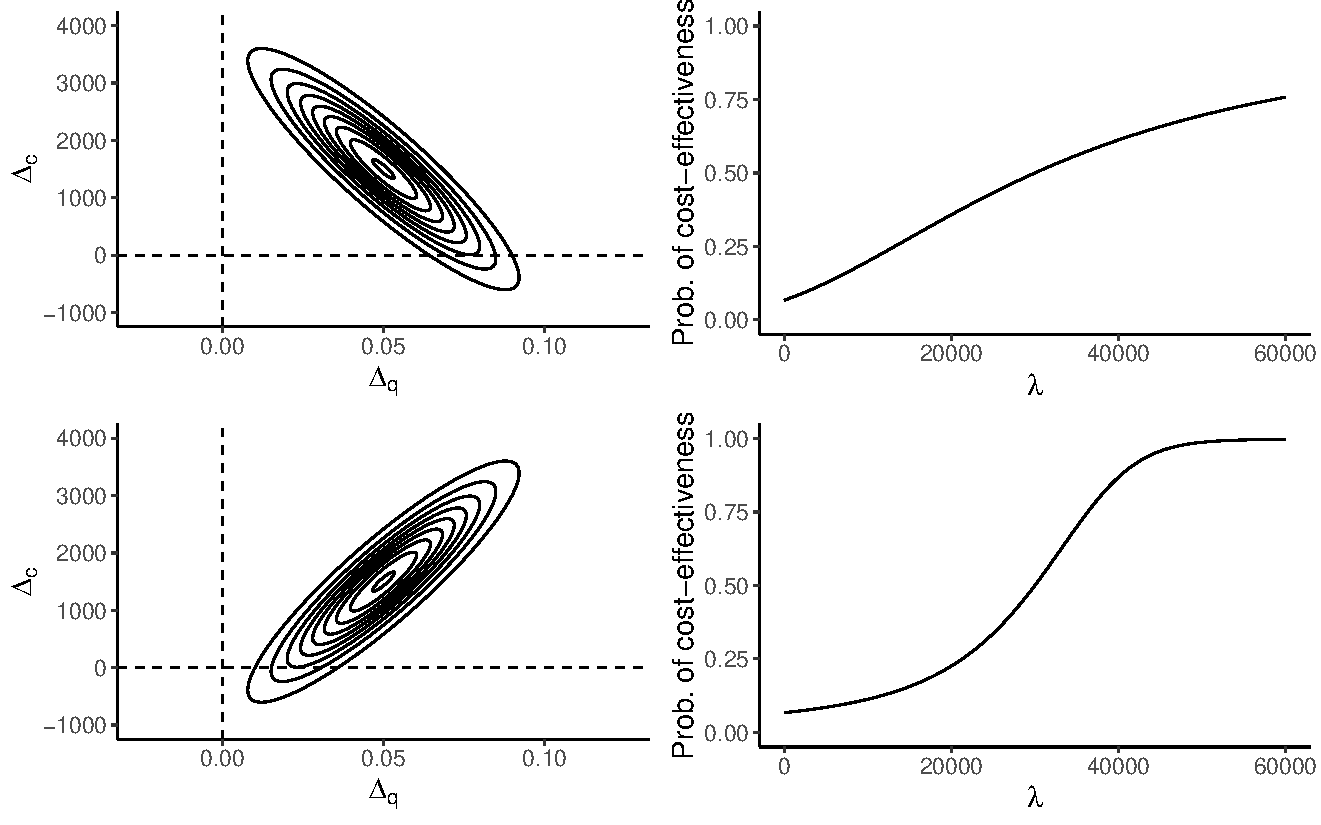
\includegraphics[width = 0.8\textwidth]{correlation_plot.pdf}
    \caption{Correlation between $\Delta_c$ and $\Delta_q$ and its impact on the probability of cost-effectiveness.}
    \label{fig:cor_illustration}
\end{figure}

\section{Observational studies and model specification}\label{sec:model_specification}

When cost-effectiveness data are obtained from a randomized trial, model specification is generally less critical. By design, treatment assignment is independent of baseline characteristics, so simple comparisons of mean costs and effects between treatment groups provide unbiased estimates of treatment effects. It is nonetheless recommended to adjust for baseline covariates to improve precision; \citep{Manca2005}; linear regression models typically perform well for this purpose \citep{lin2013agnostic}.
Without randomization, however, there will generally be certain baseline characteristics, called \emph{confounders}, which influence both the treatment choice and the outcomes (i.e. cost and health) and hence need to be adjusted for in the analysis. This adjustment necessitates the use of a statistical model, as we need to specify how exactly the confounders influence the outcomes. Even with all relevant confounders measured, a badly chosen model may lead to biased and inconsistent estimates of the treatment effects \citep{aronow2025nonparametric}, making model choice a critical matter when analysing observational data.

With that in mind, we will now critically examine some of the commonly used model choices in CEAs. A frequently used model is seemingly unrelated regression (SUR, \citet{zellner1962efficient, ben2023conducting}), which asserts that 
\begin{align}
\begin{pmatrix}  c_i \\ q_i \end{pmatrix} &= 
\begin{pmatrix}  \boldsymbol{\beta_1}^\top \mathbf{x_i}  \\ \boldsymbol{\beta_2}^\top \mathbf{x_i} \end{pmatrix} +
\begin{pmatrix}  \varepsilon_{i,1} \\ \varepsilon_{i,2} \end{pmatrix}, 
& \begin{pmatrix}  \varepsilon_{i,1} \\ \varepsilon_{i,2} \end{pmatrix} \sim \text{N}\Biggl(\begin{pmatrix}  0 \\ 0 \end{pmatrix}, \boldsymbol{\Sigma} \Biggl)
\label{eq:basic_SUR}
\end{align}

With SUR, patients’ costs $c_i$ and health outcomes $q_i$ are modeled as linear functions of a set of covariates $\mathbf{x}_i$, representing baseline characteristics or transformations thereof (which may include, say, quadratic or interaction terms), plus a bivariate-normally distributed distributed error term. In a CEA, both the linearity and the normality assumption are questionable, and we shall now scrutinize each of them in turn.

The normality assumption is rarely realistic in the CEA setting, particularly for the cost outcome, which can only take non-negative values and is often right-skewed \citep{el2022scoping}. However, violations of this assumption are not always critical: \citet{white1980heteroskedasticity} showed that, as long as certain mild conditions are met, the estimates from linear regression models (such as SUR) remain unbiased and consistent\footnote{Consistency means, roughly speaking, that with a sufficiently large sample the estimate will be close to the true value.}, even when the distribution of the error term is misspecified. Nonetheless, the normality assumption can be weakened by through the use of bootstrapping, as is frequently done in CEA \citep{lothgren2000definition}.

Another way to avoid the normality assumption, which has been promoted by many authors but not applied much in practice, is the use of generalized linear models (GLMs). Those allow the specification of non-normal error terms—for example, by modeling costs using a lognormal or gamma distribution \citep{baio2018statistical,gabrio2019bayesian}. However, this approach has a significant drawback: the results can be very sensitive to the choice of the distribution. A valuable simulation study by \citet{briggs2005parametric} showed that, if a lognormal distribution is assumed for the costs, but the true distribution is gamma, the estimated mean costs are strongly biased. The sample mean on the other hand, which is essentially a linear
regression without covariates, performs well regardless of the true distribution. The same patterns will persist in the more observational setting, with adjustment for baseline covariates. The reason is that, for GLMs with non-normal error terms, there are no theoretical guarantees analogous to those in linear models — that is, if the error term in a GLM is not specified correctly, the resulting estimates may be inaccurate even with large sample sizes. In consequence, choosing the wrong distribution for the outcome can lead to both biased and inconsistent treatment effect estimates.

A more fundamental limitation of the SUR model is the assumption of linearity. Violations of this assumption can lead to severe bias in the estimated treatment effects.
%; we illustrate this through a simple simulation experiment in Appendix~\ref{app:simulation_experiment}. 
While SUR models can be extended to include transformations of the covariates (like interactions or polynomial terms or exponential terms), this requires the analyst to correctly anticipate the relevant functional form on these transformations. This becomes increasingly challenging in high-dimensional observational settings, and does not guarantee good performance \citep{dorie2019automated}. GLMs suffer from analogous problems. For example, a GLM for costs often assumes that the logarithm of the expected costs depends linearly on the covariates \citep{baio2018statistical}; an assumption just as restrictive as the linearity in the SUR model. More generally, both SUR and GLMs are examples of parametric models, which make strong assumptions about how the covariates are related to the outcomes. Violations of these assumptions lead to biased estimates of treatment effects \citep{dorie2019automated}. 

In order to deal with the aforementioned problem, statisticians have developed regression techniques which do not make strong parametric assumptions about the relationship between the covariates and the outcomes. These so called \emph{nonparametric regression models}\footnote{The term "nonparametric" is somewhat of a misnomer, since such models do in fact have parameters. However, the number of these parameters (or more technically: the dimension of the parameter space) is not chosen in advance, unlike in, say, the linear model. Nonetheless, the terminology is widely used.} enjoy increasing popularity in the estimation of causal treatment effects; see the recent review by \citet{caron2022estimating}. Crucially, under similar regularity conditions, robustness guarantees analogous to those of linear regression  also exist for nonparametric regression models, even when the normal error distribution is misspecified \citep{kleijn2006misspecification}.
However, nonparametric regression models can be somwehat challenging to use and interpret. In particular, unlike in the basic linear model, the treatment effects of interest are no longer represented by a single model parameter, making their interpretation less straightforward for applied researchers in the absence of clear guidelines and practical explanations.

\section{BART for CEAs}
We will focus on a specific nonparametric regression model, namely \emph{Bayesian additive regression trees} (BART), which has been shown to perform well at estimating treatment effects  \citep{dorie2019automated}. 
We have recently extended this model to account for the correlation between costs and health outcomes found in CEA data; this extended version is called suBART \citep{esser2025seemingly}

As the name suggests, BART is a Bayesian statistical model and works by aggregating a set of regression trees. We shall now explain briefly what each of these terms mean. 

\subsection{Regression trees}
While regression models come in many forms, they all share the common goal of describing the relationship between an outcome variable and one or more covariates. A regression tree does this by dividing the covariate space (the set of all possible values of $\mathbf{x}_i$) into distinct "bins". Then each of these bins is assigned a single value, representing the predicted or expected outcome for all observations whose covariates fall within that bin. We illustrate this through a simple example.
%%%
\\~\\
\textbf{Example 3.} 
A representation of a simple regression tree is shown on the left of Figure~\ref{fig:tree_example}. We may imagine this tree giving us the predicted QALY for a particular patient, based on their baseline health state (expressed as a number between 0 and 1). Given a specific value for this baseline utility --- say $x$ --- how do we find the predicted QALY? We start at the top of the tree, and then move down the levels sequentially. At each step, we follow either the left or the right direction, depending on whether $x$ is smaller or larger than the shown threshold value. Once we reach the end of a branch (where the tree no longer splits), we take the given value as the predicted QALY.
We can also use the tree to plot the expected QALY as a function of $x$. This is illustrated in the right panel of Figure~\ref{fig:tree_example}. Where a linear model would have given us a line, the regression tree produces a so-called step function.
\\~\\
\begin{figure}[H]
\centering
\vspace{-0.5cm}
\begin{subfigure}[t]{0.44\textwidth}
\centering
        \begin{forest}
    for tree={
        grow=south, draw, minimum size=3ex, 
        inner sep=3pt, % control the overall tree size
        s sep=7mm,
        l sep=6mm
    }
    [$x \le 0.3$,
        [$0.2$, edge label={node[midway, left, font=\footnotesize]{TRUE\:}}, circle,]
        [$x \le 0.6$, edge label={node[midway, right, font=\footnotesize]{\:FALSE}},
            [$x \le 0.5$, edge label={node[midway, left, font=\footnotesize]{}},
                [0.9, edge label={node[midway, left, font=\footnotesize]{}}, circle,]
                [0.4, edge label={node[midway, right, font=\footnotesize]{}}, circle,]
            ]
            [0.6, edge label={node[midway, right, font=\footnotesize]{}}, circle,]
        ]
    ]
\end{forest}
\end{subfigure}
\hspace*{\fill}
\begin{subfigure}[t]{0.54\textwidth}
\centering
     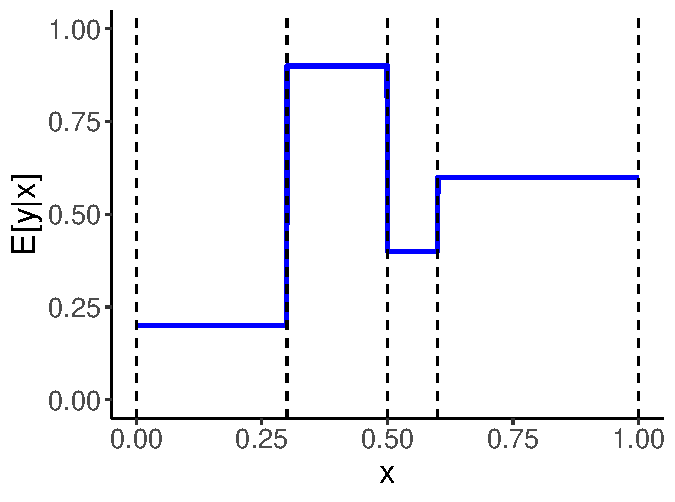
\includegraphics[width=0.8\columnwidth]{tree_example.pdf}
\end{subfigure}
\caption{Regression tree (left) and resulting regression function (right).}
\label{fig:tree_example}
\end{figure}

\subsection{BART}

The idea of the original BART model is to express the outcome as a sum of regression trees plus a normally distributed error term\footnote{As noted above, such a normally distributed error term does not pose issues even when the conditional distribution of the outcomes is not normal.}: 
\[y_i = \sum^m_{t=1} f_t\left(\mathbf{x}_i\right) + \varepsilon_i,\]
where each $f_i$ is a regression tree.
The total number of trees $m=200$ is frequently used, since this choice has been found to provide good performance while keeping the computational demands of the model fitting manageable. 
See \citet{chipman2010bart,tan2019bayesian} for detailed treatments of this model, and particularly the process by which the trees are learned from the data. \citet{hill2020bayesian} provide an overview of several extensions of BART, including models for binary regression and survival analysis.

We content ourselves here with providing some intuition for the basic BART model. A single regression tree produces a piecewise-constant approximation to the regression function: it partitions the covariate space into regions and assigns one predicted value to each region (Figure~\ref{fig:tree_example}). While this can capture sharp nonlinearities and interactions, a single tree is typically too unstable (high variance) to serve as a reliable estimator.

BART addresses this by representing the conditional mean (that is, the expected outcome given the covariates) as a sum of many shallow trees,
\[
\mathbb{E}(y_i\mid \mathbf{x}_i)\approx \sum_{t=1}^{m} f_t(\mathbf{x}_i),
\]
where each tree $f_j$ is constrained a priori to have only a few splits. Every small tree is a “weak learner" that makes only a small, local adjustment to the prediction. Adding many such adjustments yields a flexible function that can approximate nonlinear patterns and interactions without the analyst having to pre-specify them (e.g., by choosing spline functions or interaction terms manually). The Bayesian prior plays the role of \emph{regularization}: it shrinks individual tree contributions toward zero and favors simpler trees, which helps prevent overfitting.

For causal inference (as in this tutorial), the role of BART is to provide a flexible model for the conditional mean $\mathbb{E}(y_i\mid x_i)$, where the covariates $x_i$ contain a treatment indicator $t_i$. Treatment effects are then computed by \emph{g-computation}: for each unit we predict outcomes under $t_i=0$ and $t_i=1$ while holding other covariates fixed, and we average the resulting contrasts \citep{hernan2024causal}. In this sense, BART is best viewed as a flexible regression engine that (i) reduces the risk of functional-form misspecification and (ii) produces posterior draws of all derived quantities of interest (e.g., $\Delta_c$, $\Delta_q$, INB, and CEACs) in a single coherent framework.

\subsection{suBART}
The acronym suBART stands for \emph{seemingly unrelated BART}, a name deliberately reminiscent of the SUR model we described in Section \ref{sec:model_specification}. SUR consists of two linear models which are coupled through correlated error terms. suBART keeps the latter, but replaces the linear models with additive regression trees.
More precisely, the model is given by:
 \begin{align*}
\begin{pmatrix}  c_i \\ q_i \end{pmatrix} &= 
\begin{pmatrix}  \sum^m_{j = 1} f_j(\mathbf{x_i})   \\ \sum^m_{j = 1} g_j(\mathbf{x_i}) \end{pmatrix} +
\begin{pmatrix}  \varepsilon_{i,1} \\ \varepsilon_{i,2} \end{pmatrix}, 
& \begin{pmatrix}  \varepsilon_{i,1} \\ \varepsilon_{i,2} \end{pmatrix} \sim \text{N}\Biggl(\begin{pmatrix}  0 \\ 0 \end{pmatrix}, \boldsymbol{\Sigma} \Biggl),
\end{align*}
where each $f_i$ and $g_i$ is a regression tree.

As noted in Section \ref{sec:preliminaries}, costs and health outcomes are typically correlated: patients with worse health may incur higher costs, while more intensive (and expensive) care may improve outcomes. Ignoring this correlation can lead to misleading uncertainty estimates for cost-effectiveness quantities.
suBART extends standard BART by fitting two flexible regression models (one for costs and one for health outcomes) while allowing their unexplained components to be correlated. This mirrors the logic of seemingly unrelated regression, but without imposing linearity or other strong parametric assumptions on the outcome models.
The benefit of this joint modeling is not primarily in changing point estimates of $\Delta_c$ and $\Delta_q$, but in providing a more realistic joint posterior distribution. This, in turn, affects downstream quantities such as the CE plane and the cost-effectiveness acceptability curve, as discussed in Section \ref{sec:preliminaries}.

\subsection{Bayesian estimation and MCMC}
As the name suggests, BART is a Bayesian statistical method, which means that the model parameters --- and functions of these parameters, such as $\Delta_c$ --- are treated as random variables, rather than unknown constants. We learn about these parameters by examining their \emph{posterior distribution}, which quantifies how different values of the parameters are more or less likely, taking into account both prior beliefs and the evidence provided by the data. 

Bayesian estimation has a long tradition in CEA, with some authors arguing that it is the most natural framework to perform cost-effectiveness research under \citep{baio2018statistical}. One reason is that cost-effectiveness researchers are concerned with the \emph{probability of cost-effectiveness} which is nothing other than $\Pr(\lambda \Delta_q - \Delta_c > 0)$. In other words, we want to make probabilistic statements about our parameters of interest, while explicitly acknowledging uncertainty about their values, and this -- strictly speaking --- is only possible under the Bayesian paradigm. 

In addition, there are pragmatic considerations that motivate our use of Bayesian estimation. It allows for the use of complex statistical models that are computationally difficult to estimate using alternative approaches. Moreover, Bayesian estimation often performs well even when assessed by frequentist or other non-Bayesian criteria. BART is a prime example, as shown through the results of the American Causal Inference Conference (ACIC) competition \citep{dorie2019automated}.

In practice, Bayesian estimation works by taking a large number of random draws from the posterior distribution. We then use these draws to approximate our quantities of interest, such as the aforementioned probability of cost-effectiveness or confidence intervals for the treatment effects. This approximation will be quite accurate if the number of draws is sufficiently large. One popular procedure to obtain these draws is is called Markov chain Monte Carlo (MCMC), and the collection of draws is called an \emph{MCMC sample}. 
While superficially similar to bootstrapping, which is a commonly used tool in CEA, the underlying theory of MCMC is quite different. While bootstrap samples are resampled datasets used to approximate sampling variability in a frequentist framework, MCMC samples represent draws from the posterior distribution and quantify uncertainty in the parameters conditional on the observed data. In practice, however, the use of MCMC is quite similar to that of bootstrapping. For example, to construct a 90\% credible interval\footnote{The Bayesian analogue to the frequentist confidence interval.}, we can simply take the 5th and 95th percentiles of the MCMC sample.

A key difference to bootstrapping is that MCMC draws are correlated, so each successive draw depends on the one preceding it. This means that an arbitrarily starting value has to be chosen when starting the sampling, and early draws may still reflect this starting value rather than the target posterior. For this reason, it is customary to discard a number of early draws, the so called ``burn-in.'' 
Once burn-in is removed, the remaining draws can be interpreted as approximate draws from the posterior distribution. 

A large number of draws is required to ensure that summaries such as posterior means, credible intervals, or the probability of cost-effectiveness are estimated with sufficient precision. We will use $1000$ burn-in draws and $5000$ total draws later on, but this only serves as an example and is not always sufficient. 
In practice, one should at least visually inspect the MCMC draws and check whether they converged, which means that the distribution of the draws is stable over time. This can be done through a trace plot; see Appendix~\ref{app:traceplots}. Convergence can also be assessed through more quantitative measures. 
For more information on these, as well as MCMC more generally, we refer to \citet{greenberg2012introduction}, Chapter 7.
Details on the specific MCMC method for the suBART model may be found in \citet{esser2025seemingly}.

\subsection{Propensity scores}
In the causal inference literature, one frequently encounters the so-called \emph{propensity score} (PS). In observational studies, treated and untreated patients often differ systematically in their baseline characteristics. The propensity score summarizes these differences by representing the probability of receiving treatment, given observed covariates. Including the estimated propensity score as an additional covariate helps the outcome model focus on comparing patients with similar treatment probabilities. Intuitively, this encourages comparisons between ``like with like'' and reduces sensitivity to extrapolation into regions of the covariate space with little overlap \citep{hahn2020bayesian}. 

Therefore, as part of our analysis, we estimate the PS for each patient in the data, using the so-called probit BART model \citep{chipman2010bart} to predict treatment assignment based on baseline characteristics. This model differs from the outcome model in that the treatment indicator is binary, and a probit link is used internally. Conceptually, however, it serves the same purpose: flexibly capturing complex relationships between covariates and the variable of interest without requiring manual specification. The estimated PS is then included as an additional covariate when fitting the suBART model for the outcomes. This approach has been shown to perform well—and better than a suBART model without PS adjustment—in the context of observational CEAs \citep{esser2025seemingly}.

\section{Guided example}
In this section we guide the reader through the use of suBART. We use a simulated dataset, which is designed as an example and not meant to represent any specific real-world research endeavour. In the supplementary material\footnote{See \url{https://github.com/Jonas-Esser/nonparametric_CEA}}, we provide the full dataset, together with all of the following code.
The dataset contains the treatment indicator \textbf{t} (which indicates which treatment a patient received), the two outcome variables (costs and health --- represented by \textbf{c} and \textbf{q}, respectively) and the confounding variables \textbf{age}, \textbf{sex}, and \textbf{education}. For illustration, we display a subset of the data in Table~\ref{tab:data}.

\begin{table}[ht]
\caption{Subset of the simulated dataset used in the guided example. Variables include treatment ($\mathbf{t}$), outcomes ($\mathbf{c}$, $\mathbf{q}$), and covariates (\textbf{age},\textbf{sex} and \textbf{education}).}
\label{tab:data}
\centering
\begin{tabular}{rrrrrr}
\hline
\textbf{c} & \textbf{q} & \textbf{t} & \textbf{age} & \textbf{sex} & \textbf{education} \\
\hline
NA & 0.5865 & 0 & 56 & 0 & 3 \\
2882.69 & 0.9512 & 0 & 70 & 1 & 3 \\
2275.42 & 0.9149 & 0 & 71 & 1 & 3 \\
1964.08 & NA & 0 & 61 & 0 & 3 \\
2524.98 & 0.9133 & 0 & 75 & 1 & 1 \\
2683.89 & 0.6261 & 1 & 50 & 1 & 3 \\
NA & NA & 0 & 43 & 1 & 2 \\
1744.14 & 0.2123 & 1 & 21 & 1 & 3 \\
NA & 0.5122 & 1 & 28 & 0 & 3 \\
\ldots & \ldots & \ldots & \ldots & \ldots & \ldots \\
\hline
\end{tabular}
\end{table}

Some observations in the outcome variables are missing. For convenience, we proceed under the\emph{missing at random} (MAR) assumption, meaning that the probability that a value is missing does not depend on the value itself, but may depend on other observed variables (such as confounders) \citep{harel2007multiple}. BART can naturally accommodate missing outcomes under this assumption, by treating them as additional unknown quantities drawing from their posterior predictive distribution within the MCMC process, conditional on observed data and parameters. 
Intuitively, missing outcomes are predicted using information from observed covariates and from other individuals with similar characteristics. The uncertainty in these predictions is automatically carried through to the posterior distribution of all quantities of interest, including treatment effects and cost-effectiveness measures.
However, the MAR assumption is not always appropriate. The imputation feature of suBART should thus be treated a convenience rather than a guarantee of validity, and one should assess robustness to alternative missingness assumptions through sensitivity analyses, as discussed later.

If covariates are missing in an applied dataset, the workflow in this section can be combined with multiple imputation prior to model fitting; see Appendix~\ref{app:MI} for an outline of how to do this (still under the MAR assumption).

\subsection{Data formatting}
In order for the suBART code to work correctly, it is important that the data are formatted properly.
Unordered categorical variables with more than two levels (i.e., variables that represent categories without any natural order, such as blood type, region, or treatment center) should be declared as factors. In the dataset, this applies to the \texttt{education} variable. All other variables should be declared as numbers. 
Furthermore, all missing observations should be properly formatted as \texttt{NA} values, \emph{not} as text strings or numbers such as $-99$, which is occasionally observed in practice.

\begin{lstlisting}[language=R, caption={Loading the data, handling the unordered categorical variables and handle missing data in the outcomes, respectively.}]

data_url <- "https://raw.githubusercontent.com/Jonas-Esser/nonparametric_CEA/refs/heads/main/data_example_missingness.csv"
data <- read.csv(data_url)

data$education <- as.factor(data$education)
data[data == -99] <- NA
\end{lstlisting}
\subsection{Data preparation}
We put all covariates into a data frame called \texttt{X}, including the treatment indicator but \emph{not} the outcomes \texttt{c} and \texttt{q}. The \texttt{X} object should contain only those variables which are supposed to enter into the regression model, and no others.
Likewise, we put the outcomes \texttt{c} and \texttt{q} into their own data frame \texttt{Y}.

\begin{lstlisting}[language=R, caption={Construction of covariate data frame \texttt{X} and outcome data frame \texttt{Y} by selecting relevant covariates and response variables}]
X <- data[,c("t", "age", "sex", "education")]
Y <- data[,c("c", "q")]
\end{lstlisting}
\subsection{Estimation of propensity scores}\label{sec:PS}
We proceed to estimate the PS using a probit BART, where treatment assignment is modeled as a function of the previously defined confounders. While this model originates in \citet{chipman2010bart}, it is also implemented in the \texttt{subart} function, which automatically selects the probit BART model when the assigned outcome variable is binary. The number of trees and MCMC iterations was specified earlier. There are a number of other arguments that can be set for this function, related to the prior distributions of the model parameters and the workings of the sampling algorithm. Manually adjusting these arguments (often called "tuning") can sometimes lead to more accurate results, but this requires a thorough understanding of the model and its computational implementation. We thus generally recommend to stick with the default options, which have been thoroughly tested in earlier work, and refer the interested reader to \citet{chipman2010bart,esser2025seemingly} as well as the documentation within the \texttt{subart} package.

As mentioned earlier, we discard the first 1000 posterior draws (usually referred to as burn-in samples) following standard practice in the MCMC literature. This means that although we set the total number of MCMC iterations (\texttt{n\_mcmc}) to $5000$ in the code, only the remaining $4000$ samples after burn-in are used for inference.

Once estimated, we append the PS to our covariate data frame, \texttt{X}. For clarity and to keep the original data intact, we store this extended data frame in a new object called \texttt{X\_ps}.

\begin{lstlisting}[language=R, caption= {Estimation of PS by fitting a BART model using the \texttt{subart} package. When the outcome is univariate, \texttt{subart} reduces to fitting a standard BART model.}]
library(subart)

ps_fit <- subart(x_train = X[,c("age", "sex", "education")],
                 y_mat = as.matrix(X$t),
                 n_tree = 200,
                 n_mcmc = 5000,
                 n_burn = 1000)

X_ps <- X
X_ps$ps <- apply(pnorm(ps_fit$y_hat), 1, mean)
\end{lstlisting}

\subsection{Further data preparation}\label{sec:dataprep}
As mentioned above, in nonlinear models such as BART, treatment effects estimates are not represented by a single model parameter, unlike with the simple linear model without interaction terms. Instead, they  are derived from the model predictions as follows: for each patient, we estimate the expected outcomes under both treatment options and then calculate the average difference between these expected outcomes. As indicated above procedure is commonly known as \emph{g-computation}.
In a Bayesian setting, this calculation is repeated for every posterior draw, yielding full posterior distributions for treatment effects and derived quantities like the incremental net benefit.


In algorithmic form, our strategy may be outlined as follows:

\begin{enumerate}
    \item Fit the suBART model.
    \item For each patient $i$, predict according to the model:
    \begin{itemize}
        \item $\hat{c}_{i}(0)$ and $\hat{q}_{i}(0)$, which are the expected costs and QALYs of the patient, \emph{had they received treatment $0$}, regardless of the treatment they actually received. 
        \item $\hat{c_i}(1)$ and $\hat{q_i}(1)$; defined analogously.
    \end{itemize}
    \item Obtain $\Delta_c$ and $\Delta_q$ by averaging the expected values over the sample:
    $$\Delta_c = \frac{1}{n} \sum^n_{i = 1} \hat{c_i}(1) - \hat{c_i}(0)$$
    $$\Delta_q = \frac{1}{n} \sum^n_{i = 1} \hat{q_i}(1) - \hat{q_i}(0)$$
    \item Using the obtained $\Delta_c$ and $\Delta_q$, compute the incremental net benefit for any willingness-to-pay $\lambda$ of interest, through
    $$\text{INB}_{\lambda} = \lambda \Delta_q - \Delta_c$$    
\end{enumerate}
For the sake of step $3$, we create another data frame, which contains each patient twice: once with the treatment indicator set to $0$, and once with it set to $1$. This data frame is called \texttt{X\_test} in the code. 
\begin{lstlisting}[language=R, caption= {Constructing the test dataset with treatment indicators to estimate potential outcomes under both treatment and control conditions.}]
X_test <- rbind(X_ps, X_ps)
X_test$t <- c(rep(0, nrow(X)), rep(1, nrow(X)))
\end{lstlisting}

\subsection{Fitting the suBART model}
We now fit the model, using the previously constructed data frames. The comments on the model arguments from Section  \ref{sec:PS} also apply here in the same way.
\begin{lstlisting}[language=R, caption= Model fitting using suBART.] 
subart_fit <- subart(x_train = X_ps,
                        y_mat = as.matrix(Y),
                        x_test = X_test,
                        n_tree = 100,
                        n_mcmc = 5000,
                        n_burn = 1000)
\end{lstlisting}
The resulting \texttt{suBART\_fit} object contains a variety of objects; we only need the entry \texttt{suBART\_fit\$y\_hat\_test}, which corresponds to the predictions from Step \ref{sec:dataprep}. 

\subsection{Obtaining the results}
In this step, we apply the calculations from Section \ref{sec:dataprep} to all draws in the MCMC sample. We use the resulting draws of $\Delta_c$ and $\Delta_q$ to estimate $\Pr\left(\text{INB}_{\lambda} > 0\right)$ for a specified range of $\lambda$ values, which will allow us to compute and plot the cost-effectiveness acceptability curve (CEAC), as described by \citet{willan2006statistical}. 

In addition to incremental effects, CEAs often report the marginal mean costs and health outcomes in each treatment arm. Because we obtain posterior draws of the potential outcomes, these marginal means are straightforward to compute by averaging the posterior-predicted outcomes under $t=0$ and $t=1$ across individuals. This yields posterior distributions for $\mu_{c0},\mu_{c1},\mu_{q0},\mu_{q1}$, which can be summarized alongside $\Delta_c$ and $\Delta_q$.
\begin{lstlisting}[language=R, caption= {Postprocessing of MCMC sample to compute average treatment effects, construct incremental $\text{INB}_{\lambda}$ at multiple willingness-to-pay thresholds, and calculate probabilities to build the CEAC}, label=code:MCMC_sample] 
n_post <- subart_fit$mcmc$n_mcmc - subart_fit$mcmc$n_burn
subart_fit$mu <- matrix(NA, nrow = n_post, ncol = 4)
colnames(subart_fit$mu) <- c("mu_c0","mu_c1","mu_q0","mu_q1")

for (i in 1:n_post){
  subart_fit$mu[i,] <- c(
    mean(subart_fit$y_hat_test[X_test$t == 0, 1, i]),
    mean(subart_fit$y_hat_test[X_test$t == 1, 1, i]),
    mean(subart_fit$y_hat_test[X_test$t == 0, 2, i]),
    mean(subart_fit$y_hat_test[X_test$t == 1, 2, i])
  )
}

MCMC_sample <- data.frame(
  mu_c0 = subart_fit$mu[,1],
  mu_c1 = subart_fit$mu[,2],
  mu_q0 = subart_fit$mu[,3],
  mu_q1 = subart_fit$mu[,4]
)
MCMC_sample$Delta_c <- MCMC_sample$mu_c1 - MCMC_sample$mu_c0
MCMC_sample$Delta_q <- MCMC_sample$mu_q1 - MCMC_sample$mu_q0
MCMC_sample$ICER  <- ifelse(abs(MCMC_sample$Delta_q) < 1e-8, NA,
                            MCMC_sample$Delta_c / MCMC_sample$Delta_q)

lambda <- seq(0, 50000, length.out = 1000)
p <- rep(NA, length(lambda))
for (i in 1:length(lambda)){
  p[i] <- mean(lambda[i] * MCMC_sample$Delta_q - MCMC_sample$Delta_c > 0)
}
CEAC <- data.frame(lambda, p)

\end{lstlisting} 

\subsection{Plotting the results}
Finally, we plot the CE plane and CEAC, using the \texttt{ggplot2} package \citep{wickham2016ggplot}.
\begin{lstlisting}[language=R, caption= Plotting the CE plane and CEAC based on the posterior MCMC sample.]
library(ggplot2)

CEplane <- ggplot(MCMC_sample) + 
  geom_point(mapping = aes(Delta_q, Delta_c), size = 1, alpha = 0.3, show.legend = FALSE) +
  geom_point(aes(mean(Delta_q), mean(Delta_c)), color = "red", size = 2) +
  geom_vline(xintercept = 0, linetype = "dashed") +
  geom_hline(yintercept = 0, linetype = "dashed") +
  labs(x = expression(Delta[q]), y = expression(Delta[c])) +
  scale_x_continuous(limits = c(-0.05, 0.15)) +
  scale_y_continuous(limits = c(0, 1000)) +
  theme_classic() +
  theme(text = element_text(size = 14)) 

CEAC <- ggplot(data = CEAC) +
  geom_line(aes(x = lambda, y = p), linewidth = 0.8) +
  geom_vline(xintercept = 0, linetype = "dashed") +
  ylim(0,1) +
  labs(x = expression(lambda)) +
  labs(y = "Probability of cost-effectiveness") +
  theme_classic() +
  theme(text = element_text(size = 14), axis.line.y = element_blank(), legend.position = "right") +
  scale_x_continuous(label=paste0((0:5) * 10, "k")) +
  geom_vline(xintercept = 0) +
  geom_hline(yintercept = 0)

gridExtra::grid.arrange(CEplane, CEAC, nrow = 1)
\end{lstlisting}

\begin{figure}[t]
    \centering
    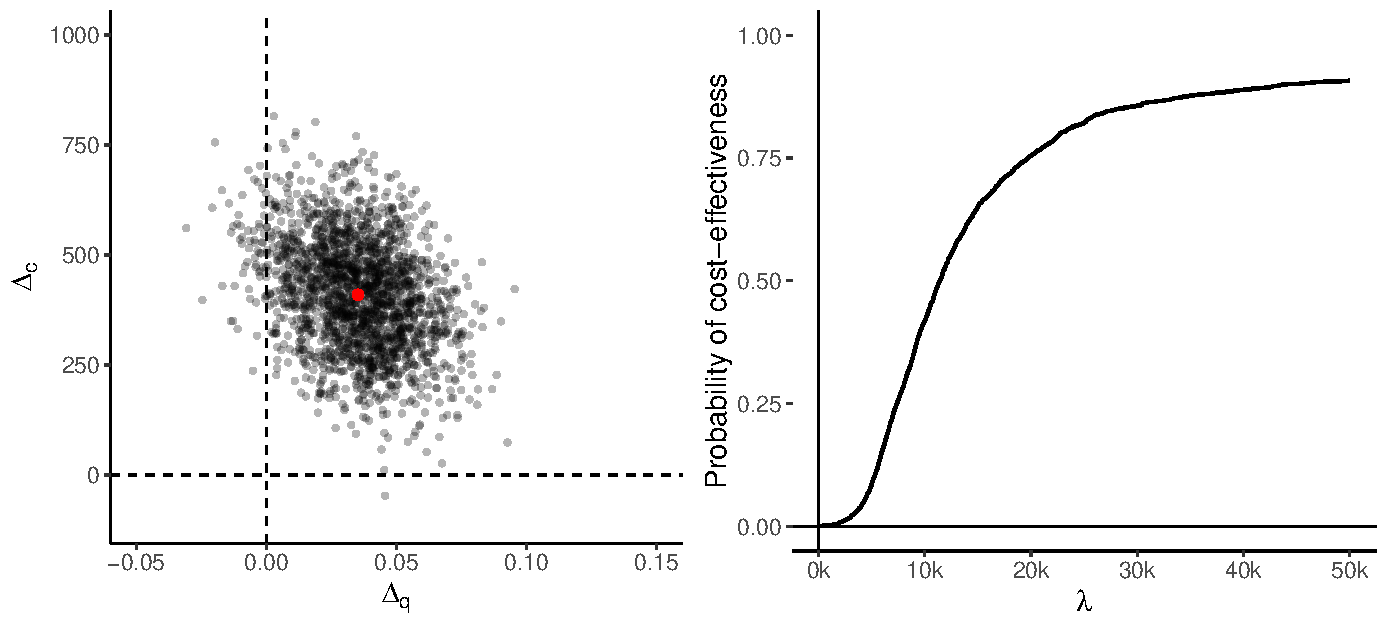
\includegraphics[width = 1\textwidth]{results_plot.pdf}
    \caption{CE plane (left) and CEAC (right).}
    \label{fig:CEplane}
\end{figure}

\section{Discussion} \label{seq:discussion}

This tutorial illustrated how flexible nonparametric regression methods can be used to estimate cost-effectiveness from observational data while accounting for complex relationships between covariates, costs, and health outcomes. The approach relies on the assumption of no unobserved confounding and is therefore most appropriate in settings where rich covariate information is available and treatment assignment is plausibly ignorable after adjustment. 


\subsection{Relation to other frameworks}
We used the suBART model in our presentation, both because of its strong empirical performance in this context and its methodological advantages. We stress, however, that our primary goal was not to advocate for one particular estimator, but to provide a general workflow for cost-effectiveness researchers analyzing observational data using nonparametric regression models.

In principle, any method that provides estimates of $\Delta_c$ and $\Delta_q$ can be used in the same way---for example, causal forests \citep{wager2018estimation} or double machine learning \citep{knaus2022double}. In a frequentist implementation, posterior draws would typically be replaced by bootstrap draws, and downstream outputs such as the CE plane and CEAC can be constructed analogously. However, the interpretation changes: in frequentist analyses, CEACs are typically based on the sampling distribution and are interpreted as measures of decision uncertainty rather than posterior probabilities; see \citet{lothgren2000definition}. In addition, bootstrap-based approaches may be challenging to use in practice due to computational demands, particularly when uncertainty must be propagated through complex postprocessing steps.

An important modeling choice concerns whether outcomes under treatment and control are estimated jointly or separately. In this tutorial, we follow a joint modeling strategy by fitting a single suBART model that includes the treatment indicator (and the propensity score) as covariates; this is an example of a so-called \emph{S-learner}. An alternative is the \emph{T-learner} approach, where we would fit separate suBART models to each treatment arm, and then obtain the treatment effects by averaging the counterfactual predictions from each model.
T-learners can be attractive when the relationship between covariates and the outcome is very different under treatment and control. However, they may suffer from higher variance in settings with limited overlap between groups (i.e., when treated and control units have very different covariate distributions) or when the sample sizes are highly unbalanced (i.e., many more observations in one group than the other).
More information T-learners, S-learners and related approaches may be found in \citet{caron2022estimating}.

Relatedly, recent work in the causal machine learning literature has promoted the use of \emph{cross-fitting} to reduce overfitting and regularization bias when flexible models are used to estimate nuisance functions (that is, intermediate quantities such as the outcome model or the propensity score which are not of primary interest but are needed to estimate treatment effects) \citep{Chernozhukov2018}. \citet{Glynn2024} apply this technique in the context of health economic decision modelling, and it might be similarly be useful for observational CEAs.
Cross-fitting involves repeatedly splitting the data into training and prediction folds, so that each observation is evaluated using models trained on separate data. While this strategy can improve robustness in large samples, it also increases computational complexity and implementation burden. For the purposes of this tutorial, we therefore focus on a single-sample approach that is easier to implement and explain, but cross-fitting could in principle be incorporated as an additional step in our proposed workflow.


\subsection{Missing data and censoring}
The suBART implementation used here can accommodate missing outcomes under the MAR assumption by drawing them from the posterior predictive distribution within the MCMC algorithm. It does not, however, directly handle missing covariates, since the model is formulated conditional on the covariates and therefore makes no assumptions about their distribution. \citet{xu2016sequential} proposed an extension of BART for imputing missing covariates under MAR. While conceptually straightforward to combine with suBART, a computational implementation would require some work.

As a pragmatic alternative, we suggest combining suBART with multiple imputation, as is commonly done in trial-based CEAs. This allows the use of suBART with missing covariates, and also with partially-observed outcomes\footnote{This may occur, for example, when the cost outcome is based on multiple self-reported questionnaires, of which some but not all have been reported by the patient.}. Concretely, one can create multiple completed datasets using standard imputation techniques and compute, for each of these datasets, posterior draws of $\Delta_c$ and $\Delta_q$. The resulting within-imputation posterior means and covariance matrices can then be pooled using Rubin's rules \citep{rubin2018multiple}. \citet{ben2023conducting} provide a specific workflow for imputation in trial-based CEAs; in our setting, their approach carries over in a straightforward manner, with posterior MCMC draws replacing bootstrap draws. For completeness, we provide a step-by-step description and example \texttt{R} code for this MI--suBART workflow in Appendix~\ref{app:MI}, designed to require only minor modifications to the analysis code presented earlier.

With respect to both outcomes and covariates, MAR is not always an appropriate assumption and should therefore be assessed through expert judgement and sensitivity analyses. For observational CEAs, these can be conducted similarly to trial-based CEAs, and the same guidance hence applies; see \citet{faria2014guide,mason2018bayesian}, for example.

Our framework also assumes that each individual's outcomes are either fully observed or entirely missing, and therefore does not directly address censoring or partially observed follow-up (e.g., due to dropout). Censoring is a long-standing challenge in cost-effectiveness analysis, particularly when costs and health outcomes accrue over time and follow-up differs between individuals. A substantial literature has developed methods to handle censoring in CEAs (e.g. \citet{lin1997estimating,bang2000estimating,willan2006statistical}), but none of them are directly compatible with the approach taken in this paper.  
\citet{sparapani2016nonparametric} have proposed a BART-based method for analysing censored data, which could in principle combined with the suBART framework, but a computational implementation would again require some work.

\subsection{Future directions}
Several extensions would broaden the applicability of nonparametric regression approaches in observational CEAs. First, methods that combine flexible outcome modeling with principled handling of missing covariates and censoring would address two common practical challenges. Second, many applications involve richer structures, such as treatment effect heterogeneity and policy-relevant subgroup effects, where tree-based Bayesian models can provide useful summaries while propagating uncertainty to cost-effectiveness outputs. Finally, extending these ideas to longitudinal and time-varying treatment settings is an important direction, although it requires additional causal assumptions and careful treatment of time-varying confounding.


%%%%%%%%%%%%%%%%%%%%%%%%%%%%%%%%%%%%%%%%%%%%%%
%% Acknowledgements                         %%
%% should be provided in the                %%
%% Acknowledgements section.                %%
%%%%%%%%%%%%%%%%%%%%%%%%%%%%%%%%%%%%%%%%%%%%%%

\section{Declarations}

\subsection{Funding}
No funding was received for the completion of this paper.

\subsection{Conflicts of interest}
All authors have no conflicts of interest to declare.

\subsection{Availability of data and materials}
All data and code used are available under \url{https://github.com/Jonas-Esser/nonparametric_CEA}.

\subsection{Ethics approval}
Not applicable.

\subsection{Author contributions}
The initial idea for the paper was proposed by Jonas Esser; the scope and design were then worked out in cooperation with Johanna van Dongen and Judith Bosmans. The text was written primarily by Jonas Esser, while incorporating suggestions from all other authors. The \texttt{R} code, figures and computer experiments were created by Jonas Esser and Mateus Maia.

%\clearpage
\interlinepenalty=1000
%\setlength{\bibsep}{3.875pt}
\bibliographystyle{ba}
\bibliography{references}

%%%%%%%%%%%%%%%%%%%%%%%%%%%%%%%%%%%%%%%%%%%%%%
%% Funding information, if any,             %%
%% should be provided in the                %%
%% funding section.                         %%
%%%%%%%%%%%%%%%%%%%%%%%%%%%%%%%%%%%%%%%%%%%%%%
% \begin{funding}
% The first author was supported by NSF Grant DMS-??-??????.

% The second author was supported in part by NIH Grant ???????????.
% \end{funding}

%%%%%%%%%%%%%%%%%%%%%%%%%%%%%%%%%%%%%%%%%%%%%%
%% Supplementary Material, including data   %%
%% sets and code, should be provided in     %%
%% {supplement} environment with title      %%
%% and short description. It cannot be      %%
%% available exclusively as external link.  %%
%% All Supplementary Material must be       %%
%% available to the reader on Project       %%
%% Euclid with the published article.       %%
%%%%%%%%%%%%%%%%%%%%%%%%%%%%%%%%%%%%%%%%%%%%%%
\clearpage
\setcounter{subsection}{0}
\renewcommand\thesubsection{\Alph{subsection}}
\renewcommand\thefigure{\thesubsection.\arabic{figure}}
\renewcommand\thetable{\thesubsection.\arabic{table}}

\section*{Appendix}\label{sec:appendix}

\subsection{Trace plots for MCMC diagnostics}\label{app:traceplots}

A trace plot visualizes how MCMC draws of a quantity evolve across iterations. It is a simple but powerful diagnostic: if the chain has converged, the trace should resemble a stable “hairy caterpillar,” fluctuating around a constant level without visible trends or structural breaks. Because our substantive targets are derived quantities such as treatment effects and incremental net benefit, it is most informative to inspect traceplots for $\Delta_c$, $\Delta_q$, and the INB directly, rather than focusing only on lower-level model parameters.

Figure~\ref{fig:traceplot} shows trace plots for the post--burn-in draws of these quantities, while the code to reproduce this figure is given in Listing \ref{code:traceplot}. The chains appear to mix well and fluctuate around stable levels without visible drift, which suggests that the chosen burn-in of $1000$ iterations is adequate in this example. We emphasize, however, that this conclusion is specific to the present dataset and model fit: in other applications, longer burn-in may be required, and traceplots should always be inspected rather than relying on default values alone.

One may ask whether convergence should also be checked for other quantities in the model, such as elements of the covariance matrix $\boldsymbol{\Sigma}$. While inspecting such lower-level parameters can be useful, especially when there are concerns about poor mixing or numerical instability, the primary inferential targets in a cost-effectiveness analysis are derived quantities such as $\Delta_c$, $\Delta_q$, and $\text{INB}_{\lambda}$. If these quantities exhibit stable traceplots and mix well after burn-in, this provides direct evidence that the posterior summaries used for decision-making are reliable.

\begin{figure}[t]
    \centering
    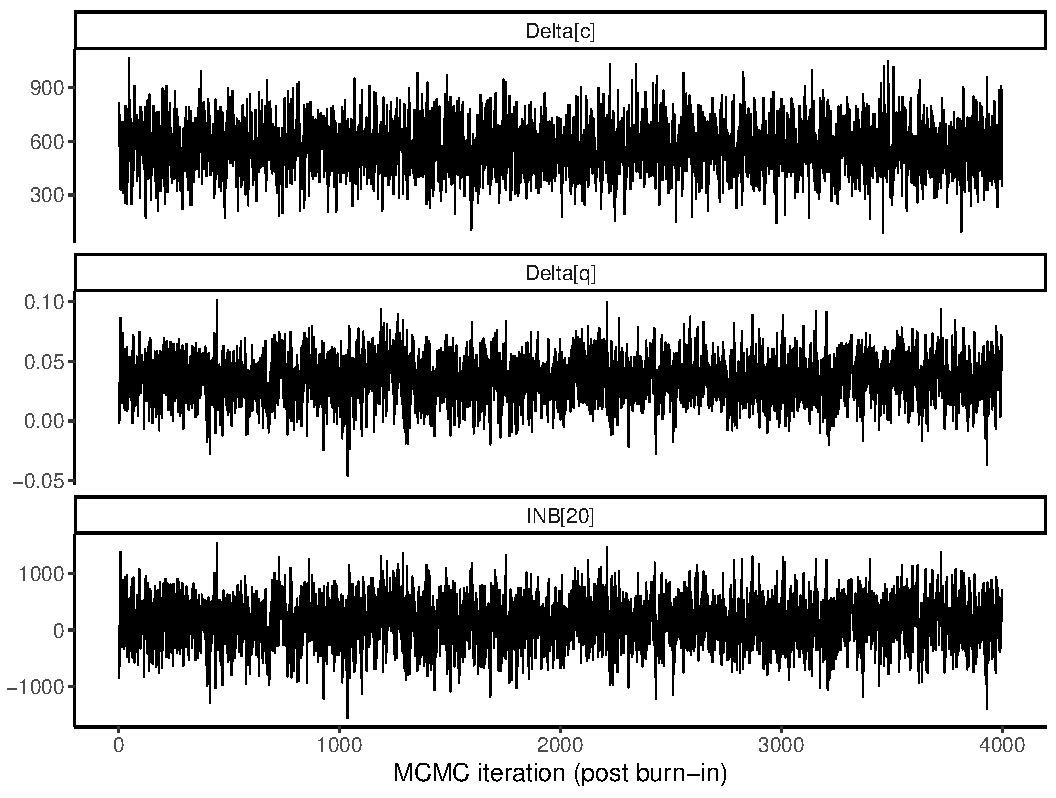
\includegraphics[width = 0.8\textwidth]{traceplot.pdf}
    \caption{Trace plots for $\Delta_c, \Delta_q$ and $\text{INB}_{20}$.}
    \label{fig:traceplot}
\end{figure}

\begin{lstlisting}[language=R, caption={Code to produce Figure \ref{fig:traceplot}.}, label=code:traceplot]
## Appendix: Traceplots for Delta_c, Delta_q, and INB20
## (Requires that the main analysis code has created `MCMC_sample`
##  with columns Delta_c and Delta_q, as in Listing 6.)

library(ggplot2)
library(tidyr)

trace_df <- data.frame(
  iter    = seq_len(nrow(MCMC_sample)),
  Delta_c = MCMC_sample$Delta_c,
  Delta_q = MCMC_sample$Delta_q,
  INB20 = MCMC_sample$INB20
)

# Convert to long format for faceting
trace_long <- pivot_longer(
  trace_df,
  cols      = c("Delta_c", "Delta_q", "INB20"),
  names_to  = "quantity",
  values_to = "value"
)

# Nice facet labels (optional)
trace_long$quantity <- factor(
  trace_long$quantity,
  levels = c("Delta_c", "Delta_q", "INB20"),
  labels = c(expression(Delta[c]), expression(Delta[q]), expression(INB[20]))
)

# Plot: 3 traceplots in one figure
ggplot(trace_long, aes(x = iter, y = value)) +
  geom_line(linewidth = 0.3) +
  facet_wrap(~ quantity, scales = "free_y", ncol = 1) +
  labs(x = "MCMC iteration (post burn-in)", y = NULL) +
  theme_classic() +
  theme(text = element_text(size = 12))


\end{lstlisting}

\subsection{Combining suBART with multiple imputation for missing covariates}
\label{app:MI}

The suBART model, like other regression-based approaches, is formulated conditional on fully observed covariates and therefore cannot directly accommodate missing covariate values. In observational CEAs, however, missing covariate data are common. A pragmatic and widely accepted solution in health economics is to combine the substantive analysis with multiple imputation (MI). In this appendix, we outline how suBART can be embedded within a standard MI workflow, closely following the approach used for trial-based CEAs by \citet{ben2023conducting}.

The key idea is to separate the handling of missing covariates from the estimation of treatment effects. Missing covariates are addressed using MI, while suBART is applied to each completed dataset. The resulting estimates are then pooled using Rubin’s rules.

\subsubsection{Outline of the procedure}
The procedure consists of the following steps:

\begin{enumerate}
    \item \textbf{Multiple imputation.}  
    Generate $M$ completed datasets using a standard MI procedure (e.g.\ the \texttt{mice} package), imputing missing covariates under a Missing At Random (MAR) assumption.

    \item \textbf{suBART estimation within each imputed dataset.}  
    For each imputed dataset $m = 1,\dots,M$, fit the suBART model exactly as described in the main text and obtain an MCMC sample of $(\Delta_c, \Delta_q)$.

    \item \textbf{Within-imputation summaries.}  
    For each imputed dataset, compute:
    \begin{itemize}
        \item the posterior mean vector
        \[
        \bar{\boldsymbol{\theta}}_m
        =
        \begin{pmatrix}
        \bar{\Delta}_{c,m} \\
        \bar{\Delta}_{q,m}
        \end{pmatrix},
        \]
        \item the posterior covariance matrix
        \(
        \mathbf{W}_m = \mathrm{Cov}_m(\Delta_c, \Delta_q),
        \)
        estimated from the MCMC draws.
    \end{itemize}

    \item \textbf{Pooling using Rubin’s rules.}  
    Combine the estimates across imputations by computing the pooled mean
    \[
    \bar{\boldsymbol{\theta}} = \frac{1}{M}\sum_{m=1}^M \bar{\boldsymbol{\theta}}_m,
    \]
    and the pooled covariance matrix
    \[
    \mathbf{T} = \mathbf{W} + \left(1 + \frac{1}{M}\right)\mathbf{B},
    \]
    where
    \[
    \mathbf{W} = \frac{1}{M}\sum_{m=1}^M \mathbf{W}_m
    \quad \text{and} \quad
    \mathbf{B} = \frac{1}{M-1}\sum_{m=1}^M
    (\bar{\boldsymbol{\theta}}_m - \bar{\boldsymbol{\theta}})
    (\bar{\boldsymbol{\theta}}_m - \bar{\boldsymbol{\theta}})^\top.
    \]

    \item \textbf{Construction of the CEAC via a normal approximation.}  
    Assuming $(\Delta_c, \Delta_q)$ is approximately bivariate normal with mean $\bar{\boldsymbol{\theta}}$ and covariance $\mathbf{T}$, the probability of cost-effectiveness for a given willingness-to-pay threshold $\lambda$ can be approximated as
    \[
    \Pr(\text{INB}_{\lambda} > 0)
    =
    \Phi\!\left(
    \frac{\lambda \bar{\Delta}_q - \bar{\Delta}_c}
         {\sqrt{\lambda^2 T_{qq} + T_{cc} - 2\lambda T_{cq}}}
    \right),
    \]
    where $\Phi(\cdot)$ denotes the standard normal cumulative distribution function.
\end{enumerate}

This approach is directly analogous to the MI--SUR--bootstrap framework described by \citet{ben2023conducting}, with posterior MCMC draws from suBART replacing bootstrap replicates from a parametric outcome model.

The normal approximation in the last step is not made out of mere convenience, but has some support in the (still developing) theory of BART: 
\citet{rockova2020semi} shows that, in the large-sample limit, the distribution of treatment effects obtained from BART models is approximately normal. Hence the pooled estimates of $\Delta_c$ and $\Delta_q$, as averages of approximately normal random variables, are again approximately normal.

\subsubsection{Example R code}
\begin{lstlisting}[language=R, caption={Illustration of combining multiple imputation with suBART using Rubin's rules.}]
library(mice)

## 1. Multiple imputation
imp <- mice(data, m = 5, method = "pmm", seed = 123)

theta_bar <- vector("list", imp$m)
W_list    <- vector("list", imp$m)

for (m in 1:imp$m) {

  ## 2. Completed dataset
  dat_m <- complete(imp, m)

  ## Re-run the suBART analysis as in the main text
  ## This produces an object `MCMC_sample_m`
  ## with columns Delta_c and Delta_q

  ## 3. Within-imputation summaries
  theta_bar[[m]] <- colMeans(MCMC_sample_m[, c("Delta_c", "Delta_q")])
  W_list[[m]]    <- cov(MCMC_sample_m[, c("Delta_c", "Delta_q")])
}

## Convert to matrix form
Theta <- do.call(rbind, theta_bar)

## 4. Rubin's rules
theta_pooled <- colMeans(Theta)

W <- Reduce("+", W_list) / imp$m
B <- cov(Theta)

T_cov <- W + (1 + 1 / imp$m) * B

## 5. CEAC via normal approximation
lambda <- seq(0, 50000, by = 500)

var_INB <- lambda^2 * T_cov[2,2] +
           T_cov[1,1] -
           2 * lambda * T_cov[1,2]

mean_INB <- lambda * theta_pooled[2] - theta_pooled[1]

CEAC <- data.frame(
  lambda = lambda,
  prob   = pnorm(mean_INB / sqrt(var_INB))
)
\end{lstlisting}

\begin{comment}

\subsection{Simulation experiment}\label{app:simulation_experiment}
We demonstrate here, through a simple simulation experiment, the consequences of model misspecification when estimating treatment effects. Such experiments are useful because we know the true data-generating process (hence also the true treatment effects) and can hence investigate how a statistical method performs at recovering the truth. The \texttt{R} code to replicate the experiment is given at the end.

The goal of our hypothetical analysis is estimating the effect of a treatment $t_i$ on the healthcare costs $c_i$, and there is a single continuous baseline covariate $x_i$. Our true model is given by 
\begin{equation*}\label{eq:true_model}
c_i = t_i + 3\sin(x_i) x_i^2 + \epsilon_i.
\end{equation*}
In line with common practice, our statistical model of choice is a simple linear regression:
\begin{equation}\label{eq:assumed_model}
c_i = \beta_0 + \beta_1 t_i + \beta_2 x_i + \epsilon_i
\end{equation}
where $\epsilon_i \sim \mathbf{N}(0,\sigma^2).$ Under the assumption of correct model specification, we have $\beta_1 = \Delta_c$.

However, our model in Equation~\eqref{eq:assumed_model} is evidently misspecified. This raises the question of what happens to our estimates when we fit model ~\eqref{eq:assumed_model} despite its  misspecification. Specifically, we ask whether the estimates can still yield meaningful information about the underlying treatment effect.

As mentioned in Section \ref{sec:model_specification}, the answer depends on whether the treatment assignment depends on the baseline covariate $x_i$. We first assign to each patient a probability of $0.5$ of receiving treatment $t_i = 1$, independently of $x_i$. The simulation setup hence mimics a randomized trial. 

We now draw $100$ random datasets from the specified simulation and analyse each dataset using the linear regression model. The left panel in Figure~\ref{fig:hist_linear} shows a histogram of the estimated treatment effects. Despite the misspecification, the estimates concentrate around the true value $1$.

\begin{figure}[htb]
    \centering
    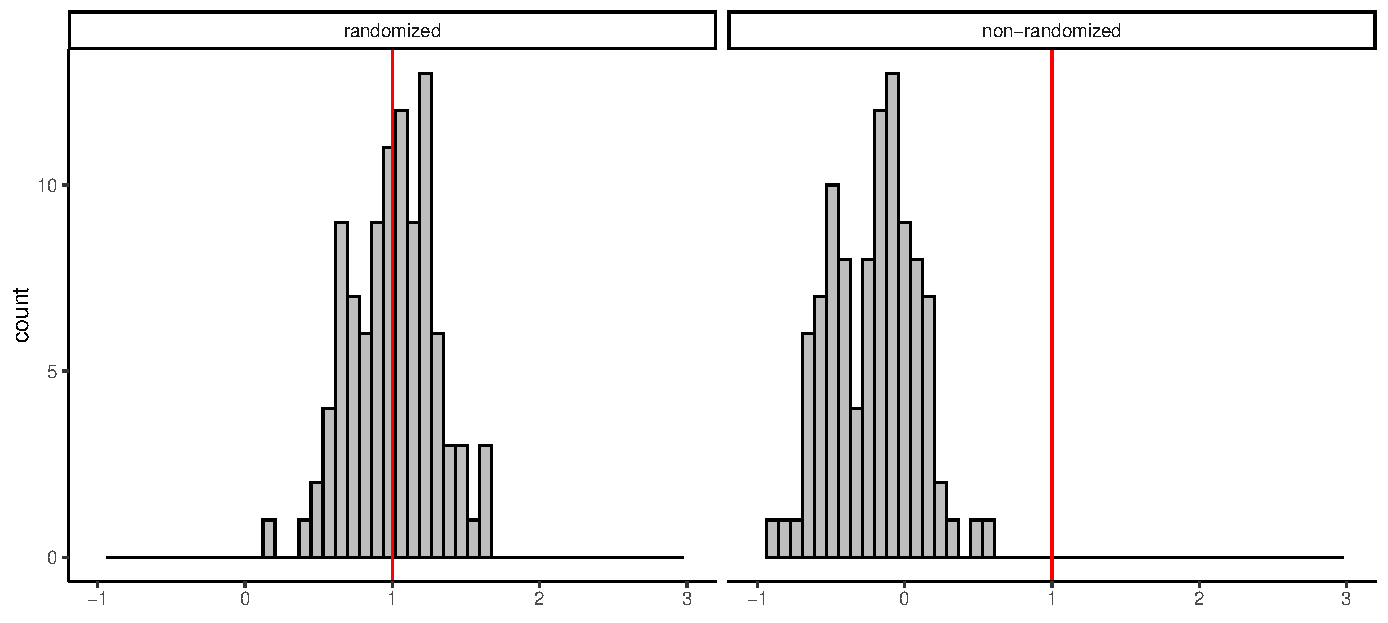
\includegraphics[width = 0.8\textwidth]{histogram_linear_model.pdf}
    \caption{Estimates of $\Delta_c$, obtained through linear regression.}
    \label{fig:hist_linear}
\end{figure}

We now modify the simulation such that $t_i$ is no longer independent of $x_i$, thereby mimicking an observational study, where the treatment assignment depends on the patients' baseline characteristics. 
\begin{equation}
    \text{Pr}(t_i = 1)= \frac{1}{1 + e^{-3x_i}}
    \label{eq:nonlinear_ps}
\end{equation}
The probability in Equation \eqref{eq:nonlinear_ps} is called the \emph{propensity score} (PS).

The results are shown in the right panel of Figure~\ref{fig:hist_linear}. Unlike before, we now observe a clear bias in the estimates. 

While our example was of course rather simplistic, the same patterns can be observed in more complex and realistic simulation experiments. A case in point is the seminal work by \citet{dorie2019automated}, where a much more elaborate and systematic simulation experiment may be found. The authors simulated data from a variety of hypothetical observational studies, using nonlinear data-generating processes. They then tasked other teams of researchers, who were unaware of the true data-generating processes, to try to estimate the average treatment effect through a statistical method of their choice. It turned out that \emph{all} variations of linear regression models performed poorly, as did other kinds of parametric models, whereas some nonparametric regression methods performed well. 

To illustrate the utility of nonparametric regression, we rerun the simulation experiment from the previous section, using BART instead of a linear regression. The results are presented in \ref{fig:hist_BART}. For each of the two data-generating processes, the inferred treatment effects concentrate around the true value, which shows that BART can correctly estimate the treatment effects even when the true relationship is nonlinear.

\begin{figure}
    \centering
    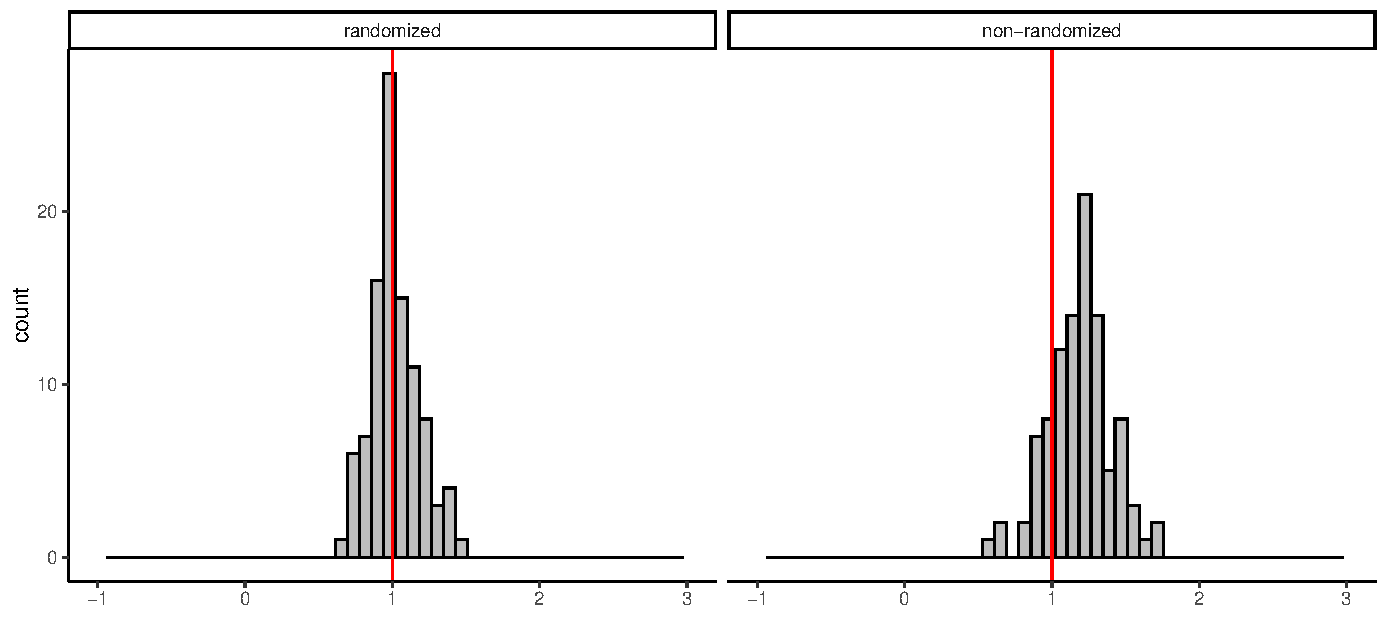
\includegraphics[width = 0.8\textwidth]{histogram_BART.pdf}
    \caption{Estimates of $\Delta_c$, obtained through BART.}
    \label{fig:hist_BART}
\end{figure}

\begin{lstlisting}[language=R, caption= {Code for the simulation experiment}]
library(subart)
library(ggplot2)

N_sim <- 100
N <- 200
X <- rnorm(N)
ATE_linear_sim1 <- rep(NA, N_sim)
ATE_linear_sim2 <- rep(NA, N_sim)
ATE_BART_sim1 <- rep(NA, N_sim)
ATE_BART_sim2 <- rep(NA, N_sim)
EY_0 <- 3 * sin(X) * X^2
EY_1 <- EY_0 + 1
ATE_true <- mean(EY_1 - EY_0)

test <- matrix(c(rep(X, 2), rep(0, N), rep(1, N)), ncol = 2)
test <- as.data.frame(test)

# sim 1: random assignment
for (i in 1:N_sim){
     A <- rbinom(N, 1, 0.5)
     Y <- (1 - A)*EY_0 + A*EY_1 + rnorm(N)
     ATE_linear_sim1[i] <- lm(Y ~ A + X)$coefficients[2]
     train <- data.frame(X,A)
     BART_mod <- subart(x_train = train,
                        y_mat = as.matrix(Y),
                        x_test = test,
                        n_tree = 100,
                        n_mcmc = 1100,
                        n_burn = 100,
                        varimportance = FALSE)
     ATE_BART_sim1[i] <- mean(BART_mod$y_hat_test_mean[(N+1):(2*N),1] - BART_mod$y_hat_test_mean[1:N,1])
}

# sim 2: nonrandom assigment
for (i in 1:N_sim){
     A <- rbinom(N, 1, 1/(1 + exp(-3*X)))
     Y <- (1 - A)*EY_0 + A*EY_1 + rnorm(N)
     ATE_linear_sim2[i] <- lm(Y ~ A + X)$coefficients[2]
     train <- data.frame(X,A)
     BART_mod <- subart(x_train = train,
                        y_mat = as.matrix(Y),
                        x_test = test,
                        n_tree = 100,
                        n_mcmc = 1100,
                        n_burn = 100,
                        varimportance = FALSE)
     ATE_BART_sim2[i] <- mean(BART_mod$y_hat_test_mean[(N+1):(2*N),1] - BART_mod$y_hat_test_mean[1:N,1])
}

data_sim <- data.frame(sim = c(rep("randomized",N_sim),rep("non-randomized",N_sim)),
                       ATE_linear = c(ATE_linear_sim1,ATE_linear_sim2),
                       ATE_BART = c(ATE_BART_sim1,ATE_BART_sim2)
)
data_sim <- data.frame(sim = c(rep("randomized",N_sim),rep("non-randomized",N_sim)),
                       ATE_linear = c(ATE_linear_sim1,ATE_linear_sim2),
                       ATE_BART = c(ATE_BART_sim1,ATE_BART_sim2)
)
data_sim$sim <- factor(data_sim$sim, levels = c("randomized", "non-randomized"))

ggplot(data_sim) +
     geom_histogram(aes(x = ATE_linear), color = "black", fill = "grey") +
     scale_x_continuous(limits = c(-1,3)) +
     geom_vline(xintercept = 1, color = "red") +
     facet_wrap(. ~ sim) +
     theme_classic() +
     theme(axis.title.x = element_blank())

ggplot(data_sim) +
     geom_histogram(aes(x = ATE_BART), color = "black", fill = "grey") +
     scale_x_continuous(limits = c(-1,3)) +
     geom_vline(xintercept = 1, color = "red") +
     facet_wrap(. ~ sim) +
     theme_classic() +
     theme(axis.title.x =  element_blank())


\end{lstlisting}
\end{comment}

\end{document}

